\vspace{1em}
% ------------------------------------------------------------------------------
% Conclusão
% ------------------------------------------------------------------------------


\chapter{Conclusão}
\label{chap_conclusao}

Para facilitar a consulta, os principais resultados gráficos discutidos nesta conclusão podem ser referenciados como: Figura~\ref{fig:comparativo_abc} (comparação dos perfis de movimento), Figura~\ref{fig:acuracia_comparativa} (acurácia dos métodos numéricos) e Tabela~\ref{tab:tabela_acuracia} (tabela comparativa de acurácia).

O estudo da queda livre, apesar de sua simplicidade aparente, mostrou-se um excelente laboratório para a aplicação e análise de métodos numéricos, modelagem matemática e validação de soluções analíticas. As simulações computacionais permitiram comparar regimes físicos distintos — sem resistência do ar, com resistência linear e quadrática — e avaliar o impacto dos parâmetros físicos e numéricos na precisão dos resultados.

Os resultados evidenciaram que a escolha do passo de tempo ($\Delta t$) é determinante para a acurácia dos métodos numéricos, especialmente em modelos com resistência do ar, que exigem discretizações mais refinadas para garantir resultados confiáveis. A comparação entre soluções numéricas e analíticas demonstrou a convergência dos métodos implementados, além de revelar limitações e potencialidades de cada abordagem.

Além de aprofundar a compreensão dos fenômenos físicos envolvidos, este trabalho reforça a importância da modelagem matemática e da análise computacional na solução de problemas reais, destacando a necessidade de escolhas criteriosas de parâmetros e validação rigorosa dos resultados.
 

\section*{Comparação dos Perfis de Movimento}


Inicialmente, foi realizado o comparativo entre as três simulações principais: queda livre sem resistência do ar, com resistência linear e com resistência quadrática. Os gráficos a seguir apresentam a evolução de posição, velocidade e aceleração ao longo do tempo para cada modelo físico:

\begin{figure}[H]
\centering
\begin{subfigure}[b]{0.32\textwidth}
\centering
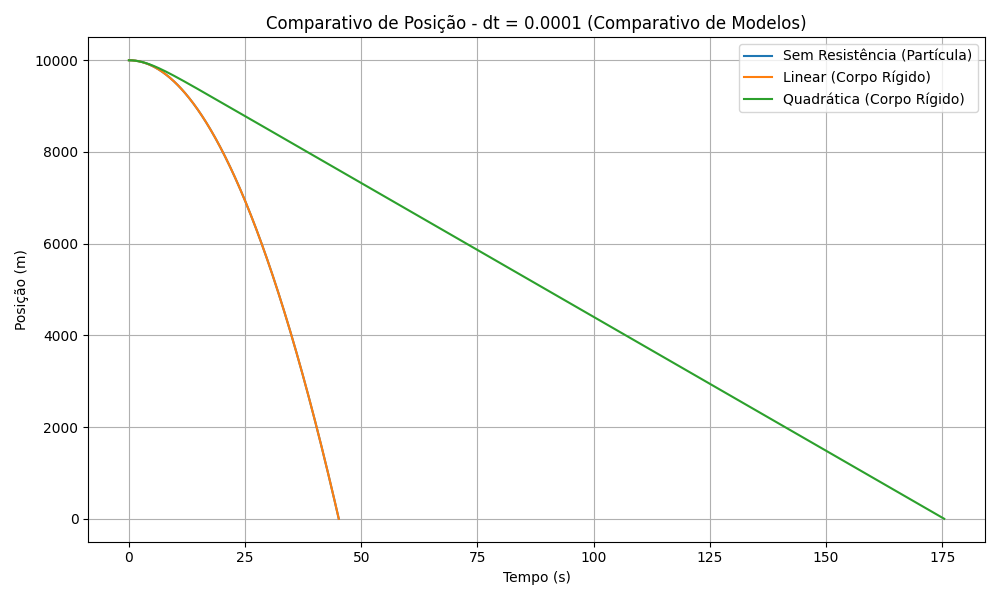
\includegraphics[width=\textwidth]{./figuras/graficos/comparativo/comparativo_posicao.png}
\caption{(a) Posição}
\label{fig:comparativo_posicao}
\end{subfigure}
\hfill
\begin{subfigure}[b]{0.32\textwidth}
\centering
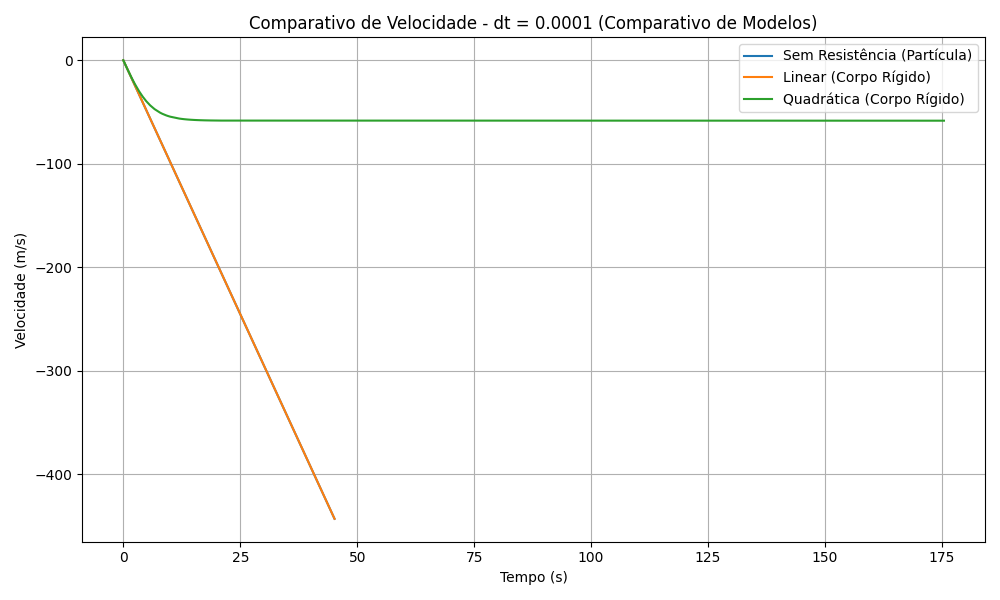
\includegraphics[width=\textwidth]{./figuras/graficos/comparativo/comparativo_velocidade.png}
\caption{(b) Velocidade}
\label{fig:comparativo_velocidade}
\end{subfigure}
\hfill
\begin{subfigure}[b]{0.32\textwidth}
\centering
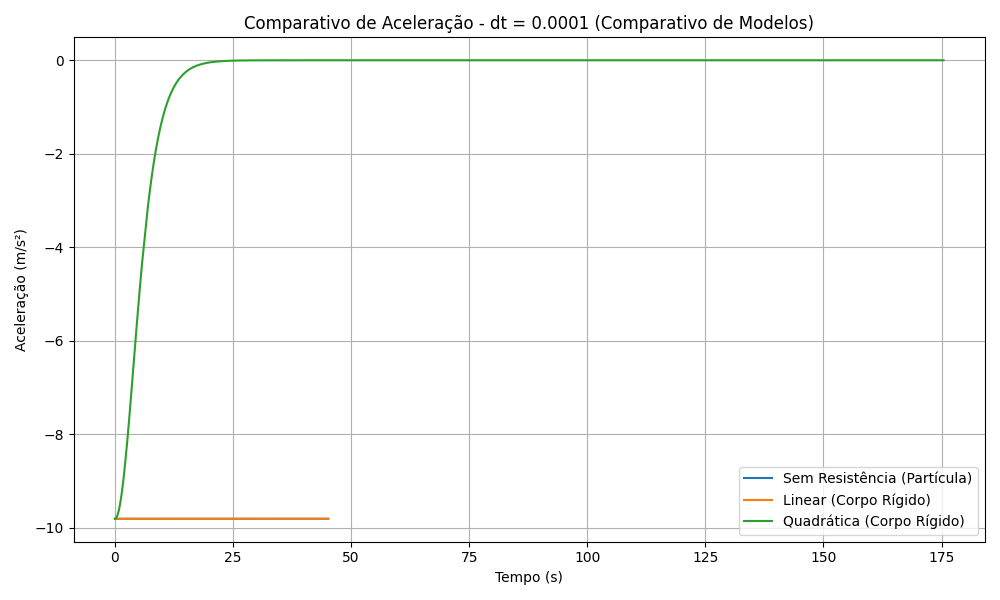
\includegraphics[width=\textwidth]{./figuras/graficos/comparativo/comparativo_aceleracao.png}
\caption{(c) Aceleração}
\label{fig:comparativo_aceleracao}
\end{subfigure}
\caption{Comparação dos perfis de (a) posição, (b) velocidade e (c) aceleração ao longo do tempo para os diferentes modelos.}
\label{fig:comparativo_abc}
\end{figure}


De modo geral, os resultados mostram que a influência do passo de tempo ($\Delta t$) é pequena para o modelo sem resistência do ar, mas torna-se cada vez mais relevante nos modelos com resistência linear e, principalmente, quadrática. Quanto maior a complexidade do regime físico, maior a necessidade de uma escolha criteriosa de $\Delta t$ para garantir precisão e estabilidade numérica. Assim, a modelagem adequada e a análise computacional cuidadosa são essenciais para obter resultados confiáveis em diferentes cenários de queda livre.

\section*{Síntese dos Resultados de Acurácia}

Na sequência, foi realizada a análise de acurácia dos métodos numéricos empregados. O gráfico a seguir ilustra o erro relativo médio para cada modelo físico e método numérico, em função do passo de tempo ($\Delta t$):

\begin{figure}[H]
	\centering
	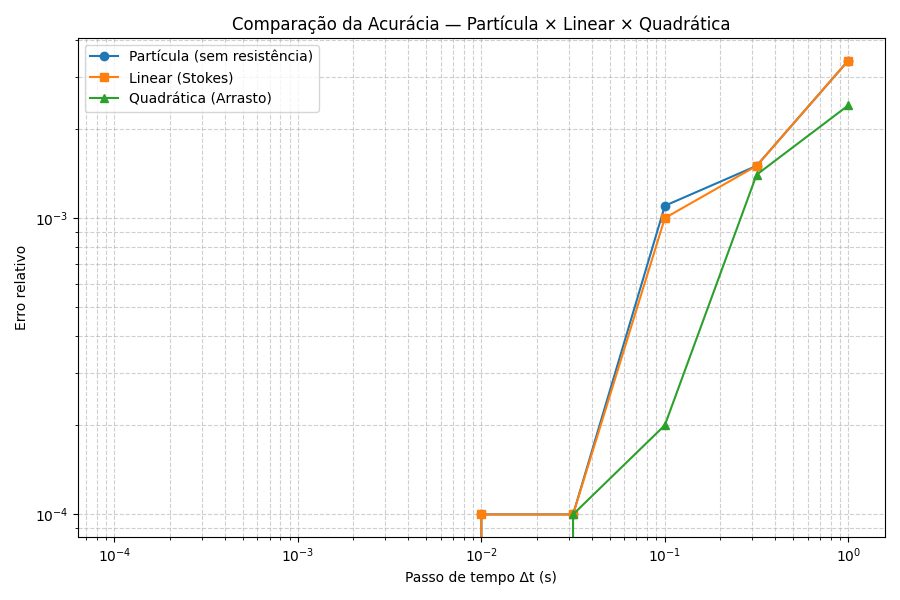
\includegraphics[width=0.6\textwidth]{./figuras/graficos/acuracia/log/acuracia_comparativa_log.png}
	\caption{Comparação do erro relativo médio entre os métodos numéricos e modelos físicos, em função de $\Delta t$.}
	\label{fig:acuracia_comparativa}
\end{figure}

Para consolidar a análise, apresenta-se a seguir a tabela comparativa de acurácia obtida nos experimentos:

\begin{center}
	\begin{table}[H]
\centering
\caption{Tabela – Dados referentes a Tabela acuracia.}
\label{tab:tabela_acuracia}

\resizebox{\textwidth}{!}{
\begin{tabular}{l l l l l l l}
\toprule
dt (s) & Tempo Final Partícula (s) & Tempo Final Linear (s) & Tempo Final Quadrática (s) & Erro Partícula & Erro Linear & Erro Quadrática \\
\midrule
0.0001 & 45.1524 & 45.1535 & 175.4286 & 0.0 & 0.0 & 0.0 \\
0.0003 & 45.1523 & 45.1535 & 175.4286 & 0.0 & 0.0 & 0.0 \\
0.001 & 45.152 & 45.154 & 175.428 & 0.0 & 0.0 & 0.0 \\
0.0032 & 45.151 & 45.1542 & 175.4274 & 0.0 & 0.0 & 0.0 \\
0.01 & 45.15 & 45.15 & 175.43 & 0.0001 & 0.0001 & 0.0 \\
0.0316 & 45.1573 & 45.1573 & 175.4115 & 0.0001 & 0.0001 & 0.0001 \\
0.1 & 45.2 & 45.2 & 175.4 & 0.0011 & 0.001 & 0.0002 \\
0.3162 & 45.2206 & 45.2206 & 175.1902 & 0.0015 & 0.0015 & 0.0014 \\
1.0 & 45.0 & 45.0 & 175.0 & 0.0034 & 0.0034 & 0.0024 \\
\bottomrule
\end{tabular}
}
\end{table}
	\label{tab:tabela_acuracia}
\end{center}


\noindent



Esses resultados quantitativos, sintetizados na tabela, evidenciam que a escolha do modelo físico impacta diretamente a precisão das variáveis simuladas. Para a partícula (sem resistência), posição, velocidade e tempo final apresentaram erros praticamente nulos, demonstrando excelente concordância com a solução analítica. No corpo rígido com resistência linear, a posição e o tempo final mantiveram alta precisão, mas a velocidade passou a apresentar pequenos desvios para passos de tempo maiores. Já no regime quadrático, a influência da resistência do ar tornou a acurácia mais sensível, especialmente para velocidade e aceleração, que exibiram erros mais perceptíveis quando $\Delta t$ foi aumentado. Portanto, conclui-se que a posição é a variável mais robusta em todos os cenários, enquanto velocidade e aceleração exigem maior atenção à escolha do passo de tempo, principalmente em modelos com resistência. Esses achados reforçam a importância de uma modelagem criteriosa e da análise comparativa entre diferentes regimes para garantir resultados confiáveis em simulações de queda livre.

